\chapter{Implementação paralelo do PSO}

Executar na Memphis outras funções (esphere, rosenbrock, rastringin)

%----------------------------------------------------------------
\section{Estratégia de paralelismo}
%----------------------------------------------------------------

Texto da seção

%----------------------------------------------------------------
\section{Topologia de comunicação}
%----------------------------------------------------------------

Texto da seção

%----------------------------------------------------------------
\section{Resultados experimentais}
%----------------------------------------------------------------

Nesta seção apresentaremos os resultados das execuções do algoritmo PSO na plataforma Memphis.
A coluna “Nº de elementos processadores” se refere à quantidade do mestre somado aos processadores escravos, exceto ao que se refere com 1 que é o algoritmo serial. Já a coluna “Tempo algoritmo (ticks)” se refere ao tempo de execução do algoritmo somente com o tempo em ticks, cada tick equivale a 10µs. A coluna “Tempo plataforma (ticks)” se refere ao tempo do algoritmo somado ao tempo da preparação da plataforma. A coluna “Speedup”
Nas tabelas abaixo estão os valores de cada execução do algoritmo na plataforma Memphis variando a população e as interações:

%-------------------------------------------------------------------------
%                               TABELAS
%-------------------------------------------------------------------------

%-------------------------------------------------------------------------
%                               20 iterações
%-------------------------------------------------------------------------

\begin{table}[h]{12cm}
    \caption{Cenário de teste com população igual a 100 e 20 iterações}
    \label{tbl:taylor-vortex-parameters}
    \begin{tabular}{llll}
        \hline
        \shortstack[l]{Nº de elementos \\ processadores} & \shortstack[l]{Tempo algoritmo \\ (ticks)} & \shortstack[l]{Tempo plataforma \\ (ticks)} & Speedup \\
        \hline
        1 & 1.615.530 & 1.617.079 & 1,00 \\
        2 & 1.950.193 & 1.951.735 & 0,83 \\
        3 & 1.024.344 & 1.025.892 &	1,58 \\
        4 & 720.708   & 722.186   & 2,24 \\
        5 & 589.084   & 590.562   & 2,74 \\
        6 & 503.492   & 504.970   & 3,21 \\
        \hline
    \end{tabular}
    %\legend{Texto da legenda. (Opcional)}
    %\source{Citação da fonte ou `O autor'. (opcional)}
\end{table}

\begin{table}[h]{12cm}
    \caption{Cenário de teste com população igual a 200 e 20 iterações}
    \label{tbl:taylor-vortex-parameters}
    \begin{tabular}{llll}
        \hline
        \shortstack[l]{Nº de elementos \\ processadores} & \shortstack[l]{Tempo algoritmo \\ (ticks)} & \shortstack[l]{Tempo plataforma \\ (ticks)} & Speedup \\
        \hline
        1 & 3.175.949 & 3.177.498 & 1,00 \\
        2 & 3.802.205 & 3.803.747 & 0,84 \\
        3 & 1.951.996 & 1.953.544 &	1,63 \\
        4 & 1.350.049 & 1.351.597 & 2,35 \\
        5 & 1.048.768 & 1.050.316 & 3,03 \\
        6 & 876.873   & 878.351   & 3,62 \\
        \hline
    \end{tabular}
    %\legend{Texto da legenda. (Opcional)}
    %\source{Citação da fonte ou `O autor'. (opcional)}
\end{table}

\begin{table}[h]{12cm}
    \caption{Cenário de teste com população igual a 300 e 20 iterações}
    \label{tbl:taylor-vortex-parameters}
    \begin{tabular}{llll}
        \hline
        \shortstack[l]{Nº de elementos \\ processadores} & \shortstack[l]{Tempo algoritmo \\ (ticks)} & \shortstack[l]{Tempo plataforma \\ (ticks)} & Speedup \\
        \hline
        1 & 4.732.875 & 4.734.424 & 1,00 \\
        2 & 5.657.594 & 5.659.136 & 0,84 \\
        3 & 2.875.817 & 2.877.365 &	1,65 \\
        4 & 1.960.693 & 1.962.241 & 2,41 \\
        5 & 1.511.697 & 1.513.245 & 3,13 \\
        6 & 1.245.103 & 1.246.651 & 3,80 \\
        \hline
    \end{tabular}
    %\legend{Texto da legenda. (Opcional)}
    %\source{Citação da fonte ou `O autor'. (opcional)}
\end{table}

\begin{table}[h]{12cm}
    \caption{Cenário de teste com população igual a 400 e 20 iterações}
    \label{tbl:taylor-vortex-parameters}
    \begin{tabular}{llll}
        \hline
        \shortstack[l]{Nº de elementos \\ processadores} & \shortstack[l]{Tempo algoritmo \\ (ticks)} & \shortstack[l]{Tempo plataforma \\ (ticks)} & Speedup \\
        \hline
        1 & 6.281.550 & 6.283.099 & 1,00 \\
        2 & 7.515.159 & 7.516.701 & 0,84 \\
        3 & 3.805.477 & 3.807.025 &	1,65 \\
        4 & 2.574.297 & 2.575.845 & 2,44 \\
        5 & 1.976.616 & 1.978.164 & 3,18 \\
        6 & 1.613.632 & 1.615.180 & 3,89 \\
        \hline
    \end{tabular}
    %\legend{Texto da legenda. (Opcional)}
    %\source{Citação da fonte ou `O autor'. (opcional)}
\end{table}

\begin{table}[h]{12cm}
    \caption{Cenário de teste com população igual a 500 e 20 iterações}
    \label{tbl:taylor-vortex-parameters}
    \begin{tabular}{llll}
        \hline
        \shortstack[l]{Nº de elementos \\ processadores} & \shortstack[l]{Tempo algoritmo \\ (ticks)} & \shortstack[l]{Tempo plataforma \\ (ticks)} & Speedup \\
        \hline
        1 & 7.844.240 & 7.845.789 & 1,00 \\
        2 & 9.373.217 & 9.374.760 & 0,84 \\
        3 & 4.736.120 & 4.737.668 &	1,66 \\
        4 & 3.202.018 & 3.203.566 & 2,45 \\
        5 & 2.440.490 & 2.442.038 & 3,21 \\
        6 & 1.984.755 & 1.986.303 & 3,95 \\
        \hline
    \end{tabular}
    %\legend{Texto da legenda. (Opcional)}
    %\source{Citação da fonte ou `O autor'. (opcional)}
\end{table}

%-------------------------------------------------------------------------
%                               30 iterações
%-------------------------------------------------------------------------

\begin{table}[h]{12cm}
    \caption{Cenário de teste com população igual a 100 e 30 iterações}
    \label{tbl:taylor-vortex-parameters}
    \begin{tabular}{llll}
        \hline
        \shortstack[l]{Nº de elementos \\ processadores} & \shortstack[l]{Tempo algoritmo \\ (ticks)} & \shortstack[l]{Tempo plataforma \\ (ticks)} & Speedup \\
        \hline
        1 & 2.391.648 & 2.393.582 & 1,00 \\
        2 & 2.869.352 & 2.870.894 & 0,83 \\
        3 & 1.491.879 & 1.493.427 &	1,60 \\
        4 & 1.035.484 & 1.037.032 & 2,31 \\
        5 & 831.658   & 833.136   & 2,88 \\
        6 & 701.940   & 703.624   & 3,41 \\
        \hline
    \end{tabular}
    %\legend{Texto da legenda. (Opcional)}
    %\source{Citação da fonte ou `O autor'. (opcional)}
\end{table}

\begin{table}[h]{12cm}
    \caption{Cenário de teste com população igual a 200 e 30 iterações}
    \label{tbl:taylor-vortex-parameters}
    \begin{tabular}{llll}
        \hline
        \shortstack[l]{Nº de elementos \\ processadores} & \shortstack[l]{Tempo algoritmo \\ (ticks)} & \shortstack[l]{Tempo plataforma \\ (ticks)} & Speedup \\
        \hline
        1 & 4.706.089 & 4.707.638 & 1,00 \\
        2 & 5.617.876 & 5.619.418 & 0,84 \\
        3 & 2.867.739 & 2.869.287 &	1,64 \\
        4 & 1.969.392 & 1.970.940 & 2,39 \\
        5 & 1.516.018 & 1.517.566 & 3,10 \\
        6 & 1.254.767 & 1.256.315 & 3,75 \\
        \hline
    \end{tabular}
    %\legend{Texto da legenda. (Opcional)}
    %\source{Citação da fonte ou `O autor'. (opcional)}
\end{table}

\begin{table}[h]{12cm}
    \caption{Cenário de teste com população igual a 300 e 30 iterações}
    \label{tbl:taylor-vortex-parameters}
    \begin{tabular}{llll}
        \hline
        \shortstack[l]{Nº de elementos \\ processadores} & \shortstack[l]{Tempo algoritmo \\ (ticks)} & \shortstack[l]{Tempo plataforma \\ (ticks)} & Speedup \\
        \hline
        1 & 7.024.437 & 7.025.986 & 1,00 \\
        2 & 8.368.147 & 8.369.689 & 0,84 \\
        3 & 4.238.051 & 4.239.599 &	1,66 \\
        4 & 2.876.310 & 2.877.858 & 2,44 \\
        5 & 2.204.034 & 2.205.582 & 3,19 \\
        6 & 1.802.087 & 1.803.635 & 3,90 \\
        \hline
    \end{tabular}
    %\legend{Texto da legenda. (Opcional)}
    %\source{Citação da fonte ou `O autor'. (opcional)}
\end{table}

\begin{table}[h]{12cm}
    \caption{Cenário de teste com população igual a 400 e 30 iterações}
    \label{tbl:taylor-vortex-parameters}
    \begin{tabular}{llll}
        \hline
        \shortstack[l]{Nº de elementos \\ processadores} & \shortstack[l]{Tempo algoritmo \\ (ticks)} & \shortstack[l]{Tempo plataforma \\ (ticks)} & Speedup \\
        \hline
        1 & 9.322.725  & 9.324.274  & 1,00 \\
        2 & 11.123.300 & 11.124.922 & 0,84 \\
        3 & 5.617.266  & 5.618.814  & 1,66 \\
        4 & 3.785.258  & 3.786.506  & 2,46 \\
        5 & 2.892.925  & 2.894.473  & 3,22 \\
        6 & 2.349.432  & 2.350.980  & 3,97 \\
        \hline
    \end{tabular}
    %\legend{Texto da legenda. (Opcional)}
    %\source{Citação da fonte ou `O autor'. (opcional)}
\end{table}

\begin{table}[h]{12cm}
    \caption{Cenário de teste com população igual a 500 e 30 iterações}
    \label{tbl:taylor-vortex-parameters}
    \begin{tabular}{llll}
        \hline
        \shortstack[l]{Nº de elementos \\ processadores} & \shortstack[l]{Tempo algoritmo \\ (ticks)} & \shortstack[l]{Tempo plataforma \\ (ticks)} & Speedup \\
        \hline
        1 & 11.643.190 & 11.644.820 & 1,00 \\
        2 & 13.880.754 & 13.882.376 & 0,84 \\
        3 & 6.995.997  & 6.997.545  & 1,66 \\
        4 & 4.717.449  & 4.718.997  & 2,47 \\
        5 & 3.581.066  & 3.582.614  & 3,25 \\
        6 & 2.900.382  & 2.901.930  & 4,01 \\
        \hline
    \end{tabular}
    %\legend{Texto da legenda. (Opcional)}
    %\source{Citação da fonte ou `O autor'. (opcional)}
\end{table}

%-------------------------------------------------------------------------
%                               40 iterações
%-------------------------------------------------------------------------

\begin{table}[h]{12cm}
    \caption{Cenário de teste com população igual a 100 e 40 iterações}
    \label{tbl:taylor-vortex-parameters}
    \begin{tabular}{llll}
        \hline
        \shortstack[l]{Nº de elementos \\ processadores} & \shortstack[l]{Tempo algoritmo \\ (ticks)} & \shortstack[l]{Tempo plataforma \\ (ticks)} & Speedup \\
        \hline
        1 & 3.165.517 & 3.167.066 & 1,00 \\
        2 & 3.787.460 & 3.789.002 & 0,84 \\
        3 & 1.958.955 & 1.960.503 &	1,62 \\
        4 & 1.350.337 & 1.351.885 & 2,34 \\
        5 & 1.074.999 & 1.076.547 & 2,94 \\
        6 & 900.399   & 901.877   & 3,52 \\
        \hline
    \end{tabular}
    %\legend{Texto da legenda. (Opcional)}
    %\source{Citação da fonte ou `O autor'. (opcional)}
\end{table}

\begin{table}[h]{12cm}
    \caption{Cenário de teste com população igual a 200 e 40 iterações}
    \label{tbl:taylor-vortex-parameters}
    \begin{tabular}{llll}
        \hline
        \shortstack[l]{Nº de elementos \\ processadores} & \shortstack[l]{Tempo algoritmo \\ (ticks)} & \shortstack[l]{Tempo plataforma \\ (ticks)} & Speedup \\
        \hline
        1 & 6.235.133 & 6.236.682 & 1,00 \\
        2 & 7.431.111 & 7.432.653 & 0,84 \\
        3 & 3.781.978 & 3.783.526 &	1,65 \\
        4 & 2.588.680 & 2.590.228 & 2,41 \\
        5 & 1.983.270 & 1.984.818 & 3,14 \\
        6 & 1.632.105 & 1.633.653 & 3,82 \\
        \hline
    \end{tabular}
    %\legend{Texto da legenda. (Opcional)}
    %\source{Citação da fonte ou `O autor'. (opcional)}
\end{table}

\begin{table}[h]{12cm}
    \caption{Cenário de teste com população igual a 300 e 40 iterações}
    \label{tbl:taylor-vortex-parameters}
    \begin{tabular}{llll}
        \hline
        \shortstack[l]{Nº de elementos \\ processadores} & \shortstack[l]{Tempo algoritmo \\ (ticks)} & \shortstack[l]{Tempo plataforma \\ (ticks)} & Speedup \\
        \hline
        1 & 9.310.226  & 9.311.775  & 1,00 \\
        2 & 11.076.869 & 11.078.491 & 0,84 \\
        3 & 5.600.291  & 5.601.839  & 1,66 \\
        4 & 3.790.819  & 3.792.367  & 2,46 \\
        5 & 2.896.281  & 2.897.829  & 3,21 \\
        6 & 2.358.590  & 2.360.138  & 3,95 \\
        \hline
    \end{tabular}
    %\legend{Texto da legenda. (Opcional)}
    %\source{Citação da fonte ou `O autor'. (opcional)}
\end{table}

\begin{table}[h]{12cm}
    \caption{Cenário de teste com população igual a 400 e 40 iterações}
    \label{tbl:taylor-vortex-parameters}
    \begin{tabular}{llll}
        \hline
        \shortstack[l]{Nº de elementos \\ processadores} & \shortstack[l]{Tempo algoritmo \\ (ticks)} & \shortstack[l]{Tempo plataforma \\ (ticks)} & Speedup \\
        \hline
        1 & 12.361.637 & 12.363.266 & 1,00 \\
        2 & 14.729.113 & 14.730.734 & 0,84 \\
        3 & 7.427.058  & 7.428.606  & 1,66 \\
        4 & 4.995.090  & 4.996.638  & 2,47 \\
        5 & 3.808.108  & 3.809.656  & 3,25 \\
        6 & 3.084.966  & 3.086.514  & 4,01 \\
        \hline
    \end{tabular}
    %\legend{Texto da legenda. (Opcional)}
    %\source{Citação da fonte ou `O autor'. (opcional)}
\end{table}

\begin{table}[h]{12cm}
    \caption{Cenário de teste com população igual a 500 e 40 iterações}
    \label{tbl:taylor-vortex-parameters}
    \begin{tabular}{llll}
        \hline
        \shortstack[l]{Nº de elementos \\ processadores} & \shortstack[l]{Tempo algoritmo \\ (ticks)} & \shortstack[l]{Tempo plataforma \\ (ticks)} & Speedup \\
        \hline
        1 & 15.439.550 & 15.441.180 & 1,00 \\
        2 & 18.384.023 & 18.385.646 & 0,84 \\
        3 & 9.253.339  & 9.254.887  & 1,67 \\
        4 & 6.232.248  & 6.233.796  & 2,48 \\
        5 & 4.721.028  & 4.722.576  & 3,27 \\
        6 & 3.815.373  & 3.816.921  & 4,05 \\
        \hline
    \end{tabular}
    %\legend{Texto da legenda. (Opcional)}
    %\source{Citação da fonte ou `O autor'. (opcional)}
\end{table}

%-------------------------------------------------------------------------
%                               50 iterações
%-------------------------------------------------------------------------

\begin{table}[h]{12cm}
    \caption{Cenário de teste com população igual a 100 e 50 iterações}
    \label{tbl:taylor-vortex-parameters}
    \begin{tabular}{llll}
        \hline
        \shortstack[l]{Nº de elementos \\ processadores} & \shortstack[l]{Tempo algoritmo \\ (ticks)} & \shortstack[l]{Tempo plataforma \\ (ticks)} & Speedup \\
        \hline
        1 & 3.939.130 & 3.940.679 & 1,00 \\
        2 & 4.704.341 & 4.708.553 & 0,84 \\
        3 & 2.425.787 & 2.427.335 &	1,62 \\
        4 & 1.665.306 & 1.666.854 & 2,37 \\
        5 & 1.318.249 & 1.319.797 & 2,99 \\
        6 & 1.098.792 & 1.100.340 & 3,58 \\
        \hline
    \end{tabular}
    %\legend{Texto da legenda. (Opcional)}
    %\source{Citação da fonte ou `O autor'. (opcional)}
\end{table}

\begin{table}[h]{12cm}
    \caption{Cenário de teste com população igual a 200 e 50 iterações}
    \label{tbl:taylor-vortex-parameters}
    \begin{tabular}{llll}
        \hline
        \shortstack[l]{Nº de elementos \\ processadores} & \shortstack[l]{Tempo algoritmo \\ (ticks)} & \shortstack[l]{Tempo plataforma \\ (ticks)} & Speedup \\
        \hline
        1 & 7.763.052 & 7.764.601 & 1,00 \\
        2 & 9.246.037 & 9.247.579 & 0,84 \\
        3 & 4.696.389 & 4.697.937 &	1,65 \\
        4 & 3.207.139 & 3.208.687 & 2,42 \\
        5 & 2.450.316 & 2.451.864 & 3,17 \\
        6 & 2.009.146 & 2.010.694 & 3,86 \\
        \hline
    \end{tabular}
    %\legend{Texto da legenda. (Opcional)}
    %\source{Citação da fonte ou `O autor'. (opcional)}
\end{table}

\begin{table}[h]{12cm}
    \caption{Cenário de teste com população igual a 300 e 50 iterações}
    \label{tbl:taylor-vortex-parameters}
    \begin{tabular}{llll}
        \hline
        \shortstack[l]{Nº de elementos \\ processadores} & \shortstack[l]{Tempo algoritmo \\ (ticks)} & \shortstack[l]{Tempo plataforma \\ (ticks)} & Speedup \\
        \hline
        1 & 11.594.212 & 11.596.841 & 1,00 \\
        2 & 13.784.014 & 13.785.635 & 0,84 \\
        3 & 6.962.254  & 6.963.802  & 1,67 \\
        4 & 4.705.656  & 4.707.204  & 2,46 \\
        5 & 3.587.669  & 3.589.217  & 3,23 \\
        6 & 2.915.521  & 2.917.069  & 3,98 \\
        \hline
    \end{tabular}
    %\legend{Texto da legenda. (Opcional)}
    %\source{Citação da fonte ou `O autor'. (opcional)}
\end{table}

\begin{table}[h]{12cm}
    \caption{Cenário de teste com população igual a 400 e 50 iterações}
    \label{tbl:taylor-vortex-parameters}
    \begin{tabular}{llll}
        \hline
        \shortstack[l]{Nº de elementos \\ processadores} & \shortstack[l]{Tempo algoritmo \\ (ticks)} & \shortstack[l]{Tempo plataforma \\ (ticks)} & Speedup \\
        \hline
        1 & 15.399.723 & 15.401.352 & 1,00 \\
        2 & 18.332.980 & 18.334.601 & 0,84 \\
        3 & 9.237.387  & 9.238.935  & 1,67 \\
        4 & 6.205.400  & 6.206.948  & 2,48 \\
        5 & 4.723.163  & 4.724.711  & 3,26 \\
        6 & 3.820.284  & 3.821.832  & 4,03 \\
        \hline
    \end{tabular}
    %\legend{Texto da legenda. (Opcional)}
    %\source{Citação da fonte ou `O autor'. (opcional)}
\end{table}

\begin{table}[h]{12cm}
    \caption{Cenário de teste com população igual a 500 e 50 iterações}
    \label{tbl:taylor-vortex-parameters}
    \begin{tabular}{llll}
        \hline
        \shortstack[l]{Nº de elementos \\ processadores} & \shortstack[l]{Tempo algoritmo \\ (ticks)} & \shortstack[l]{Tempo plataforma \\ (ticks)} & Speedup \\
        \hline
        1 & 19.235.575 & 19.237.202 & 1,00 \\
        2 & 22.885.567 & 22.887.187 & 0,84 \\
        3 & 11.510.217 & 11.511.845 & 1,67 \\
        4 & 7.746.771  & 7.748.319  & 2,48 \\
        5 & 5.860.508  & 5.862.056  & 3,28 \\
        6 & 4.730.160  & 4.731.708  & 4,07 \\
        \hline
    \end{tabular}
    %\legend{Texto da legenda. (Opcional)}
    %\source{Citação da fonte ou `O autor'. (opcional)}
\end{table}

%-------------------------------------------------------------------------
%                               GRÁFICOS
%-------------------------------------------------------------------------

\begin{graph}[h]{16cm}
    \caption{Cenário de teste com 20 iterações}
        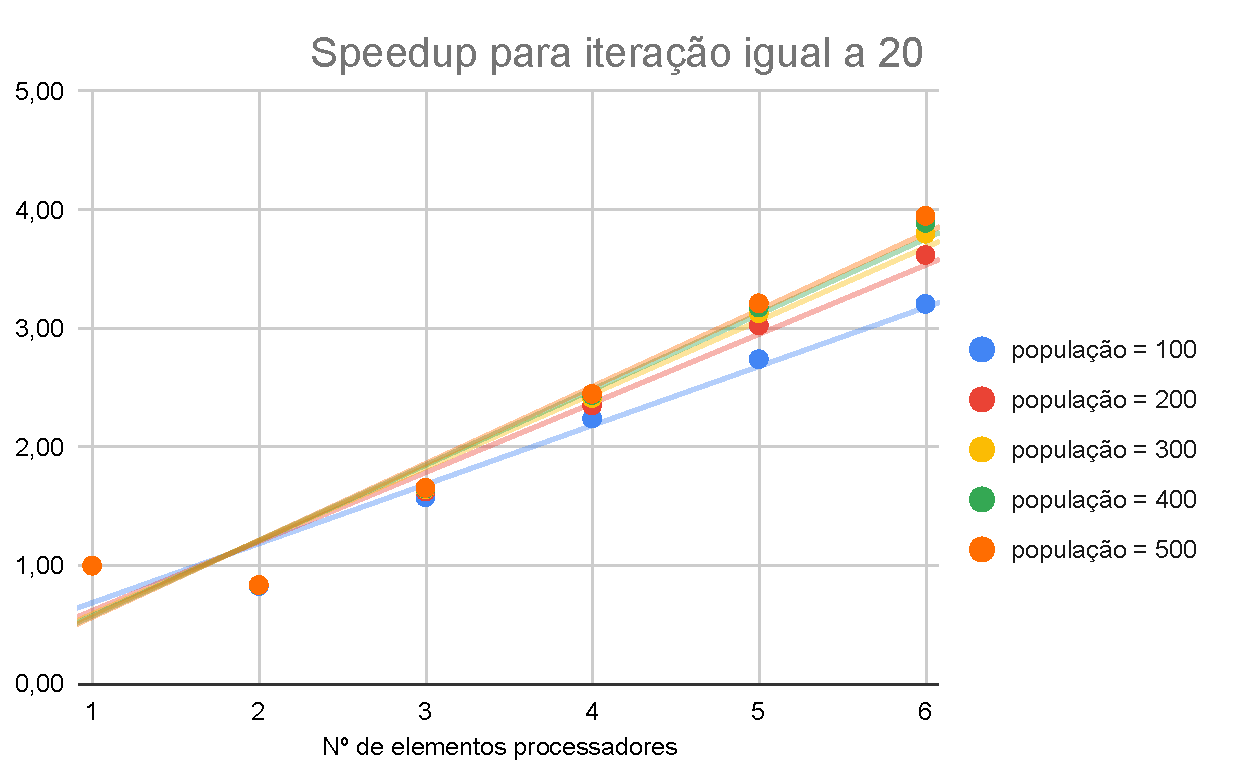
\includegraphics[width=14cm]{graficos/Speedup para iteração igual a 20.pdf}
\end{graph}

\begin{graph}[h]{16cm}
    \caption{Cenário de teste com 30 iterações}
        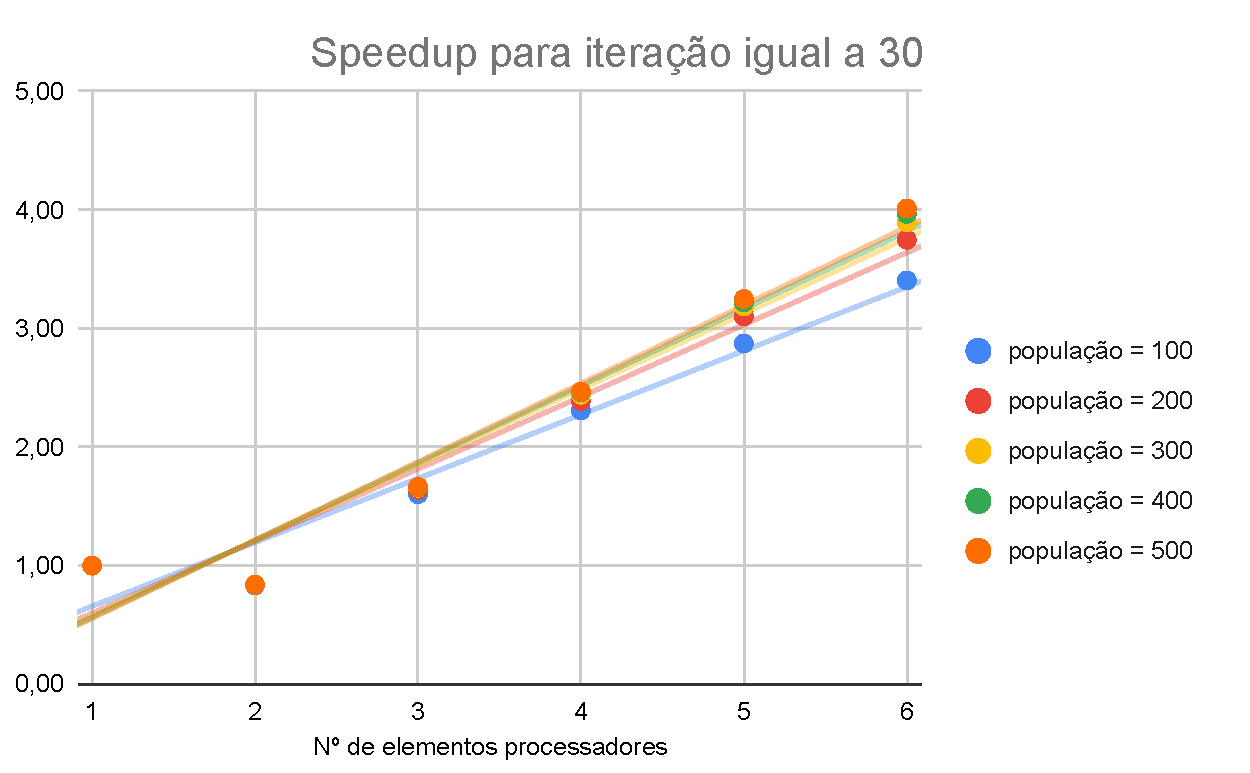
\includegraphics[width=14cm]{graficos/Speedup para iteração igual a 30.pdf}
\end{graph}

\begin{graph}[h]{16cm}
    \caption{Cenário de teste com 40 iterações}
        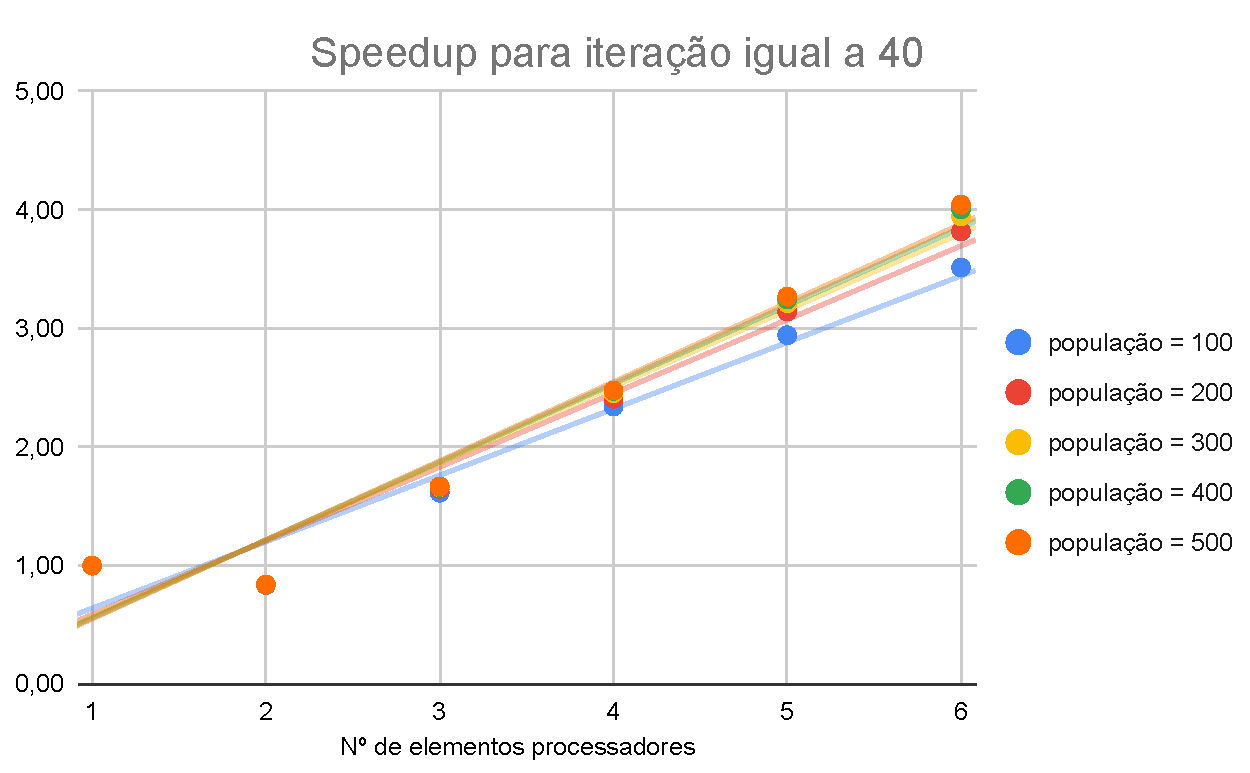
\includegraphics[width=14cm]{graficos/Speedup para iteração igual a 40.pdf}
\end{graph}

\begin{graph}[h]{16cm}
    \caption{Cenário de teste com 50 iterações}
    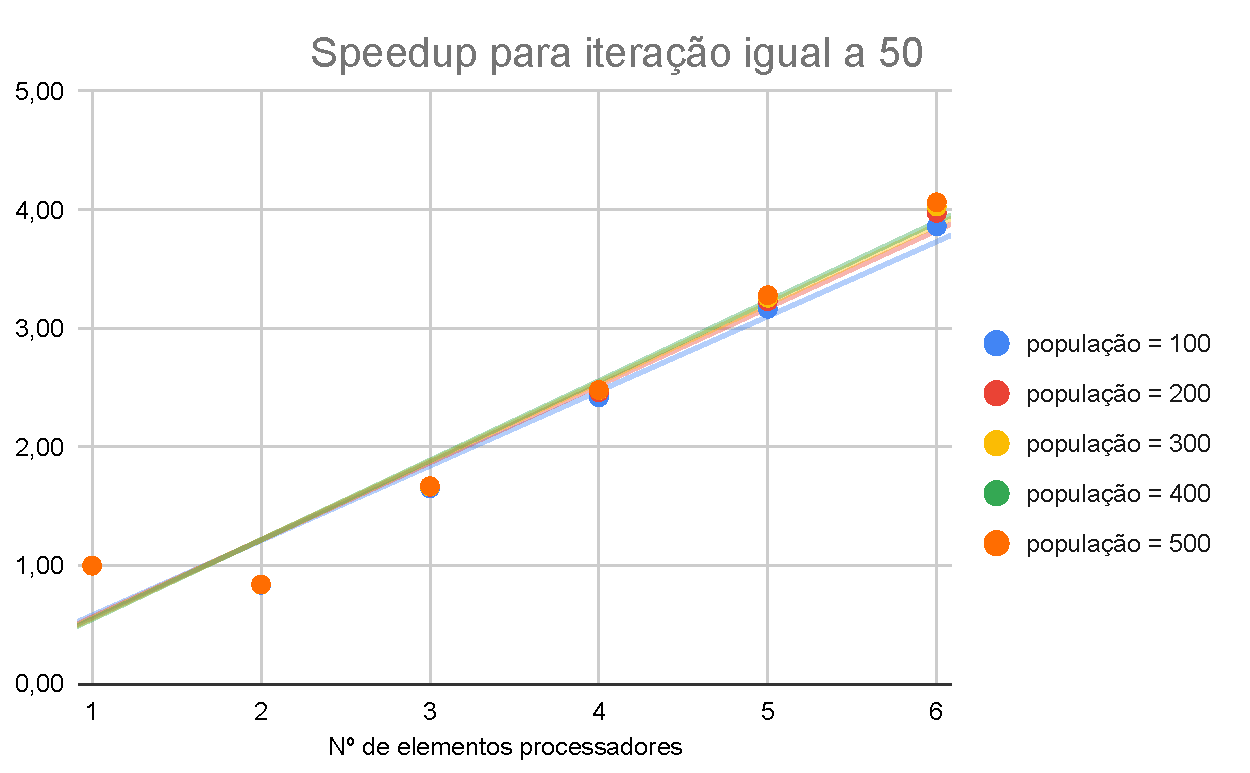
\includegraphics[width=14cm]{graficos/Speedup para iteração igual a 50.pdf}
\end{graph}

%\begin{figure}[ht]{12cm}
%  \begin{center}
%    \leavevmode
%    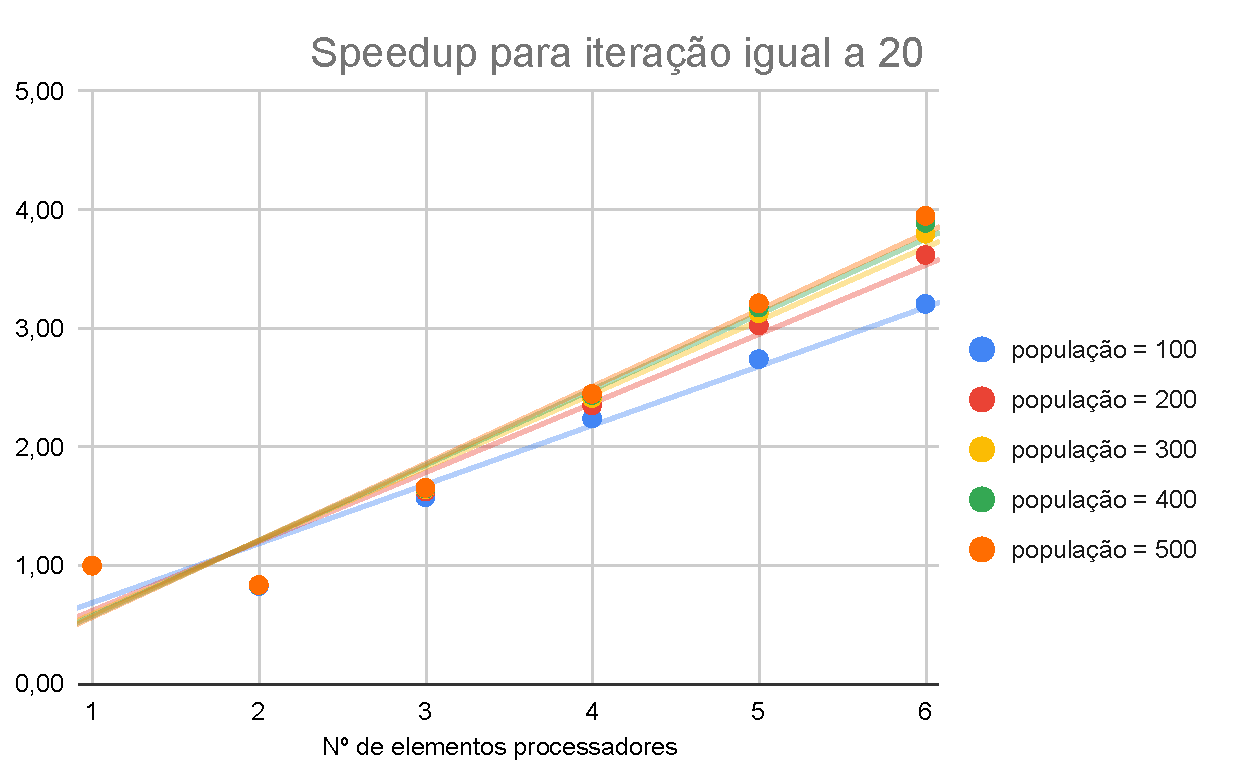
\includegraphics[width=0.65\textwidth]{graficos/Speedup para iteração igual a 20.pdf}
%    \caption{Two element linear array (from \cite{gross15})}
%    \label{fig:2elem}
%  \end{center}
%\end{figure}

Lei de Amdahl

\begin{align}
    &G=\frac{1}{S+\frac{1-S}{n}}
\end{align}